\section*{تقسیم‌بندی پروژه}
\subsection*{انتخاب
	\lr{opcode}ها}
ابتدا لیست
\lr{opcode}های
\lr{JVM}
را پیداکردیم. از آنجایی که قرار بود این پروژه برای ۵ تیم باشد، نیاز بود تا تعدادی از آپکدها را جداکنیم که پروژه برای ۴ تیم مناسب شود.
برای جداکردن تعدادی از این
\lr{opcode}ها
از
\lr{Jazelle}
الگو می‌گیریم. 
\lr{Jazelle}
به این صورت عمل می‌کند که
\lr{JVM}
دستوراتش را به
\lr{Jazelle}
می‌فرستد و اگر
\lr{Jazelle}
از آن‌ها پشتیبانی کرد، آن‌ها را اجرا می‌کند، و اگر هم پشتیبانی نمی‌کرد آن‌ها را به
\lr{JVM}
باز می‌گرداند تا آن‌ها را به دستوراتی که
\lr{Jazelle}
از آن‌ها پشتیبانی می‌کند تبدیل کند.
\begin{figure}[H]
	\centering
	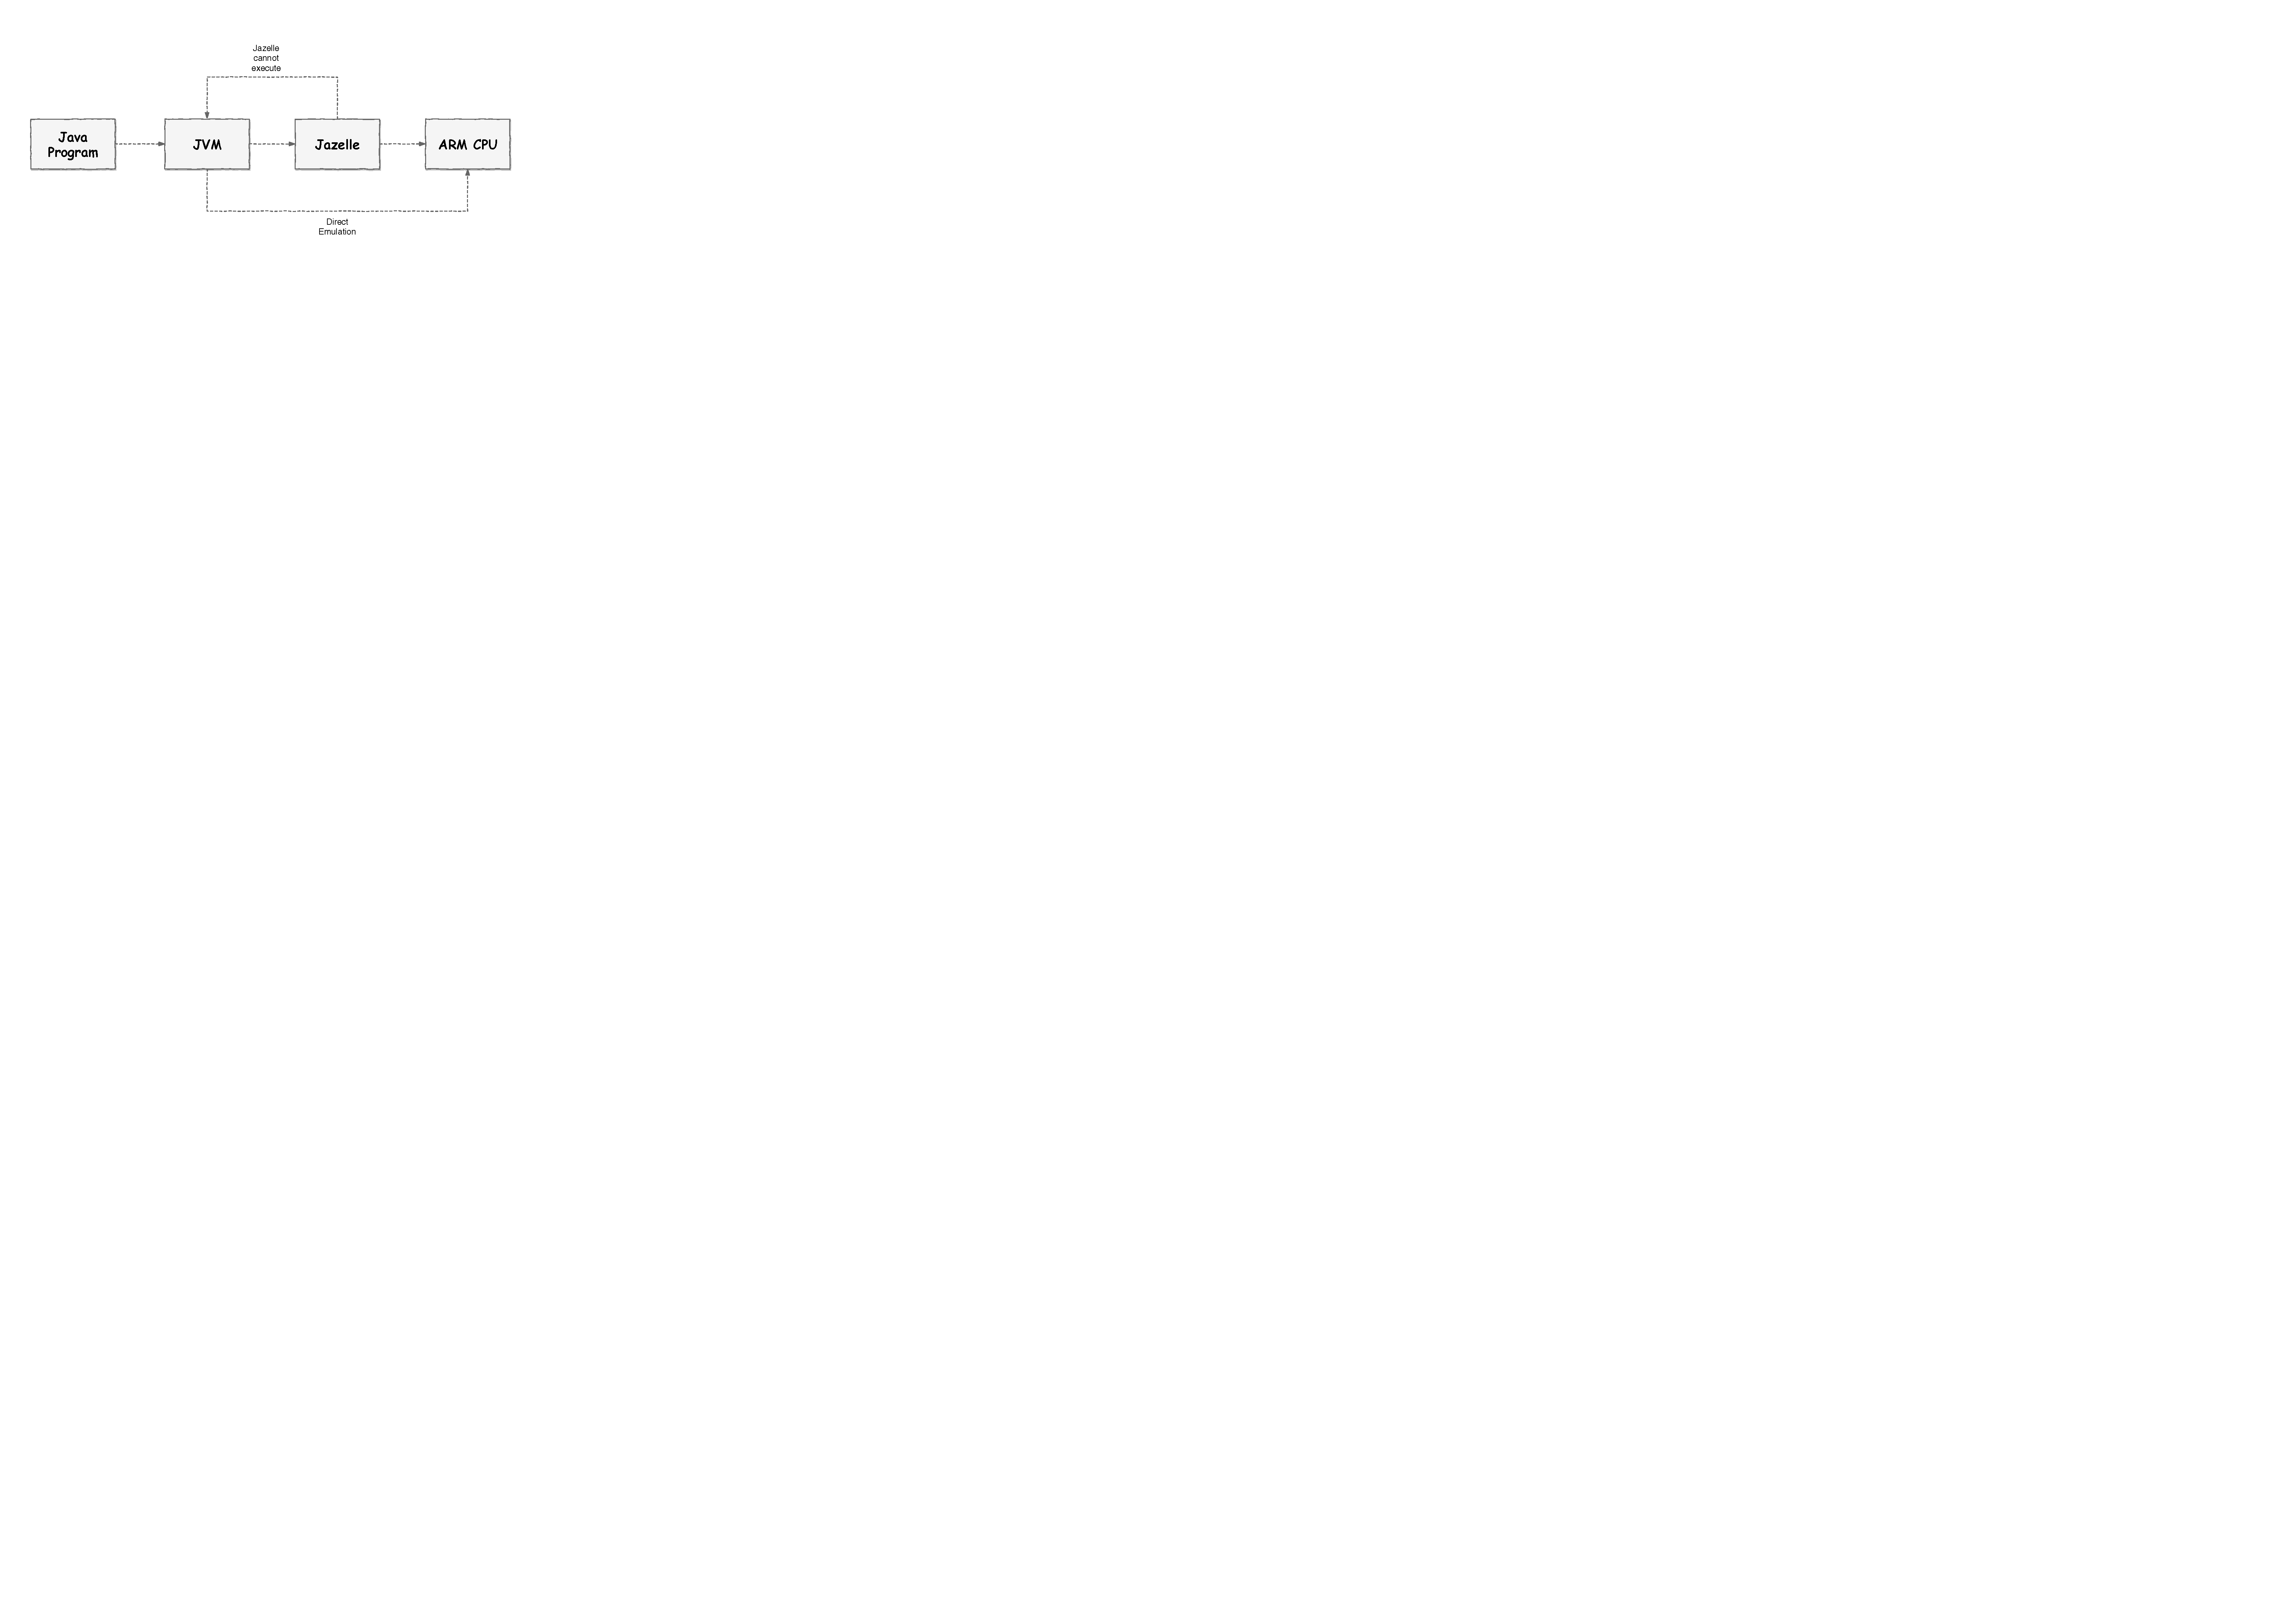
\includegraphics[width=\linewidth]{flowchart}
	\caption{روند اجرای کار jazelle}
	\label{fig:flowchart}
\end{figure}

ما نیز به این صورت عمل می‌کنیم که عده‌ای از 
\lr{opcode}ها
که پیاده‌سازی نرم‌افزاریشان ساده‌تر است را جدا می‌کنیم و الباقی
\lr{opcode}ها 
را در پیاده‌سازیمان می‌آوریم.
\subsection*{تقسیم‌بندی 
	\lr{opcode}ها
}
برای افزایش بازدهی گروه‌ها
\lr{opcode}های
انتخابی به شانزده بسته‌ی ۱۰تایی تقسیم‌بندی شدند و با یک کد 
\lr{R}
که به صورت رندوم این ۱۶ بسته را به گروه‌ها تخصیص می‌داد، تقسیم‌بندی کردیم.(سید را هم با حضور اعضای سایر گروه‌ها تعیین‌کردیم.)
\subsubsection*{کد}
\begin{latin}
	\begin{lstlisting}
	library(dplyr)
	set.seed(1919)
	s = sample(seq(from = 1, to = 16), replace = F)  
	c("jaferian", "asadi", "hoseini", "ghafarloo") %>% 
	cbind(t(apply(matrix(s, nrow = 4), 1, sort)))
	\end{lstlisting}
\end{latin}
\subsubsection*{خروجی کد}
\begin{latin}
	\centering
	\begin{tabular}{l|cccc}
		Group Name & & & & \\
		\hline \hline
		jaferian & 4 & 6 & 7 & 8\\
		
		asadi & 3 & 9 & 10 & 12\\
		hoseini & 1 & 5 & 11 & 14\\
		ghafarloo & 2 & 13 & 15 & 16\\
	\end{tabular}
\end{latin}
\subsubsection*{لیست دستورات}
لیست دستورات را می‌توانید در صفحه‌گسترده‌ی ۱ و ۲ مشاهده‌کنید.
